\providecommand{\topdir}{..}
\documentclass[../main.tex]{subfiles}

%External sources
\graphicspath{{\topdir/img/A02/}}

\begin{document}
\label{chap:control}

In April 2021 \textit{Delegación de Alumnos ETSIST-UPM} organized a microcontroller competition. The author of this project participated with a very basic physical control panel for this vision mixer. Due to its tight relation with this project, a short report about the prototype is enclosed.\newline

\section{Overview}
In the context of linear \gls{tv} production equipment, a physical panel is a must for medium to large size productions, as it allows rapid interaction with the crucial parts of the system. Vision mixers are not an exception to this rule, so a prototype of a physical control panel has been developed that allows controlling the mixer described in this end-of-degree project.\newline


Most commercial control panels feature dedicated sections for the cross-point and the transitions. More often than not, they also allow performing configurations related to the keyers. However, the prototype displayed in the figure \ref{fig:control_panel_proto} does not enable the user to perform very complex tasks. It only features a 8 channel crosspoint and two buttons to perform transitions and cuts, with no \textit{t-bar}. However, this comparison is not fair, as the \gls{bom} of it costs around $100 \si{\EUR}$, including the micro-controller, which corresponds to the $70 \si{\%}$ of the budget. As opposed to this, full-featured commercial solutions may cost orders of magnitude more.\newline

Due to the multi-client nature of the mixer, the absence of some controls on this panel is not a major problem, as the rest of the configuration is still available in the web control software. Therefore, the most used controls are easily reachable in a physical control panel, whilst the rest of the configuration may be done though the web-app.\newline

\begin{figure}[hbtp]
    \centering
    \subfigure[Chopped shot]{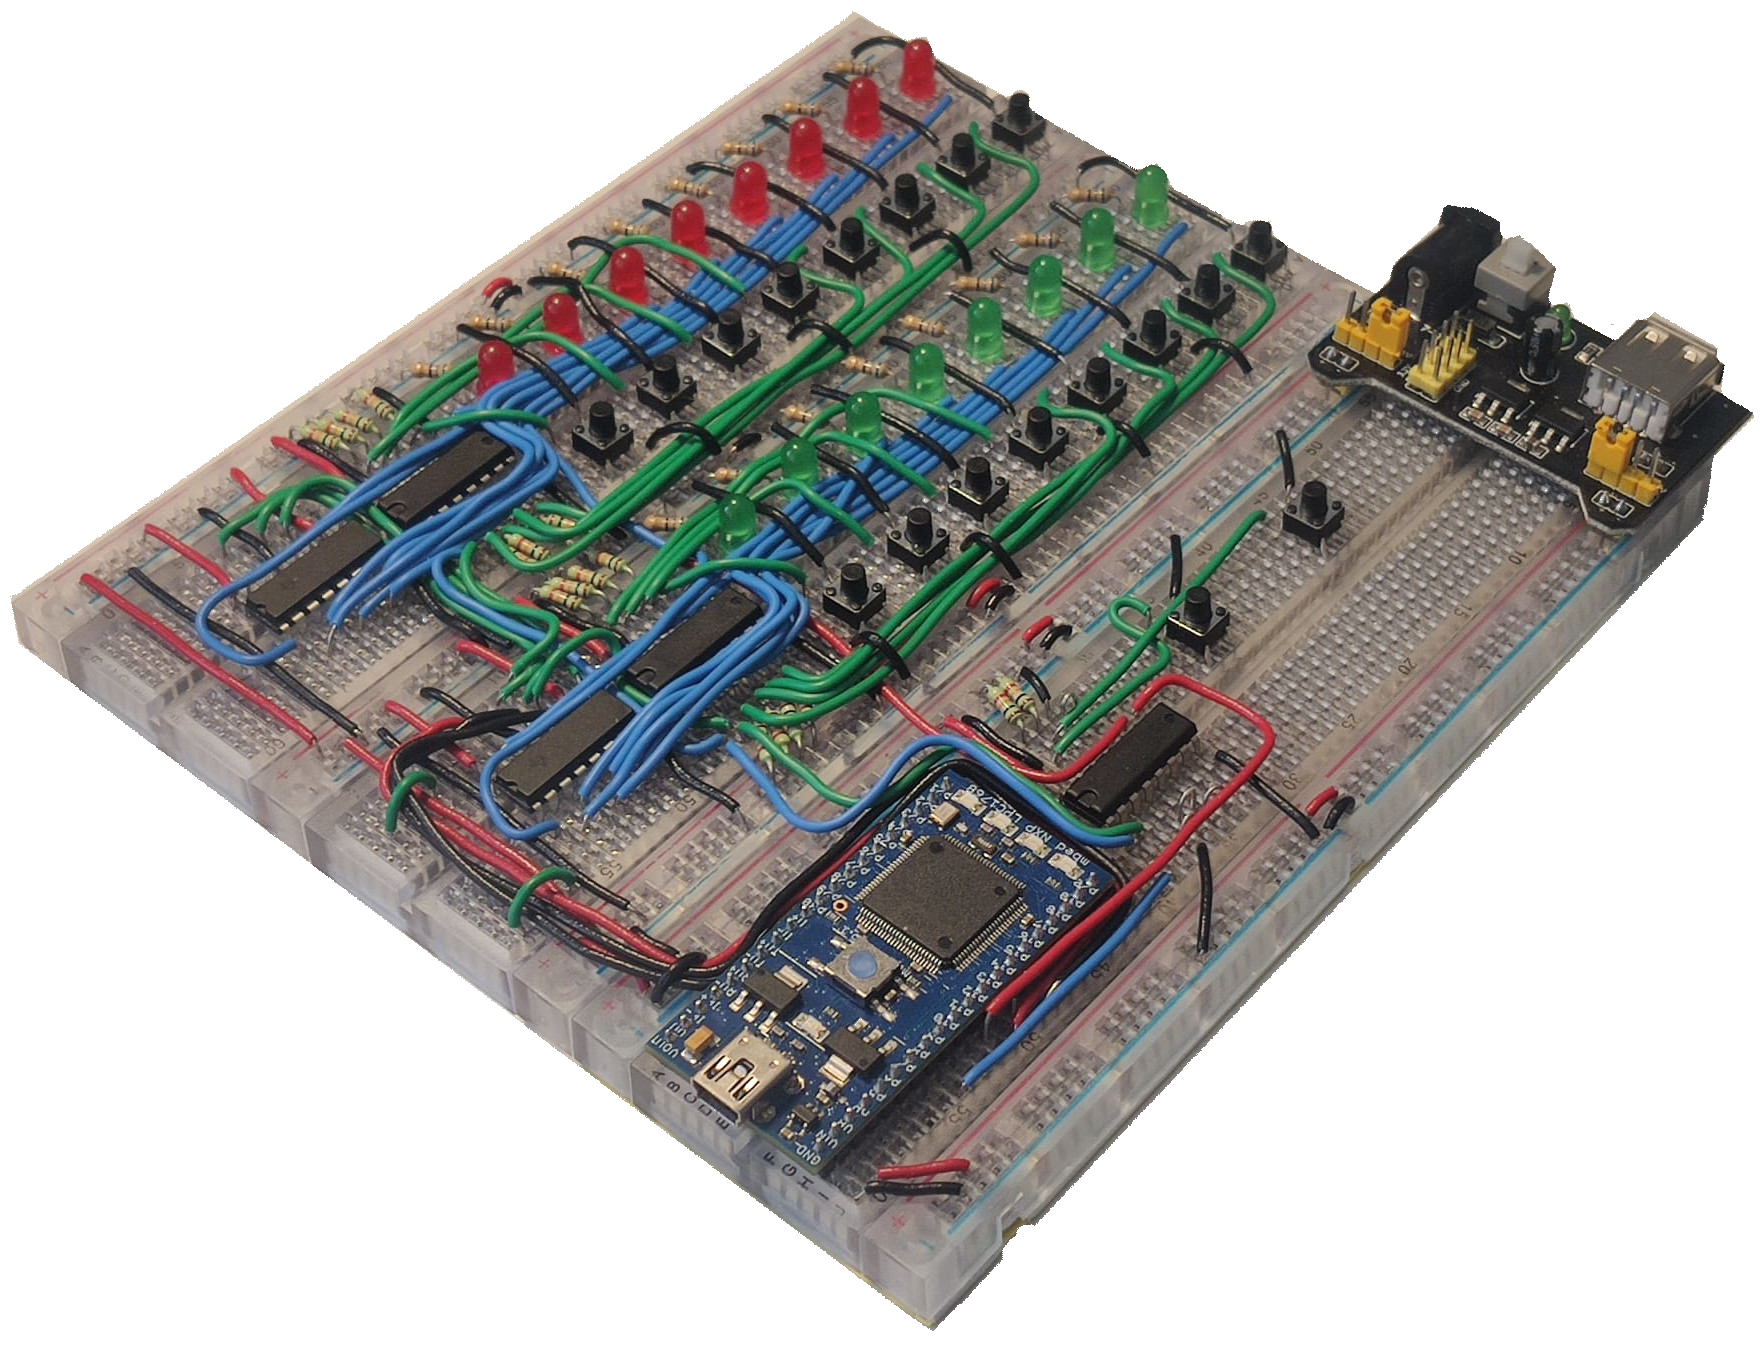
\includegraphics[width=.8\textwidth]{Chopped}}
    \subfigure[Cenital shot]{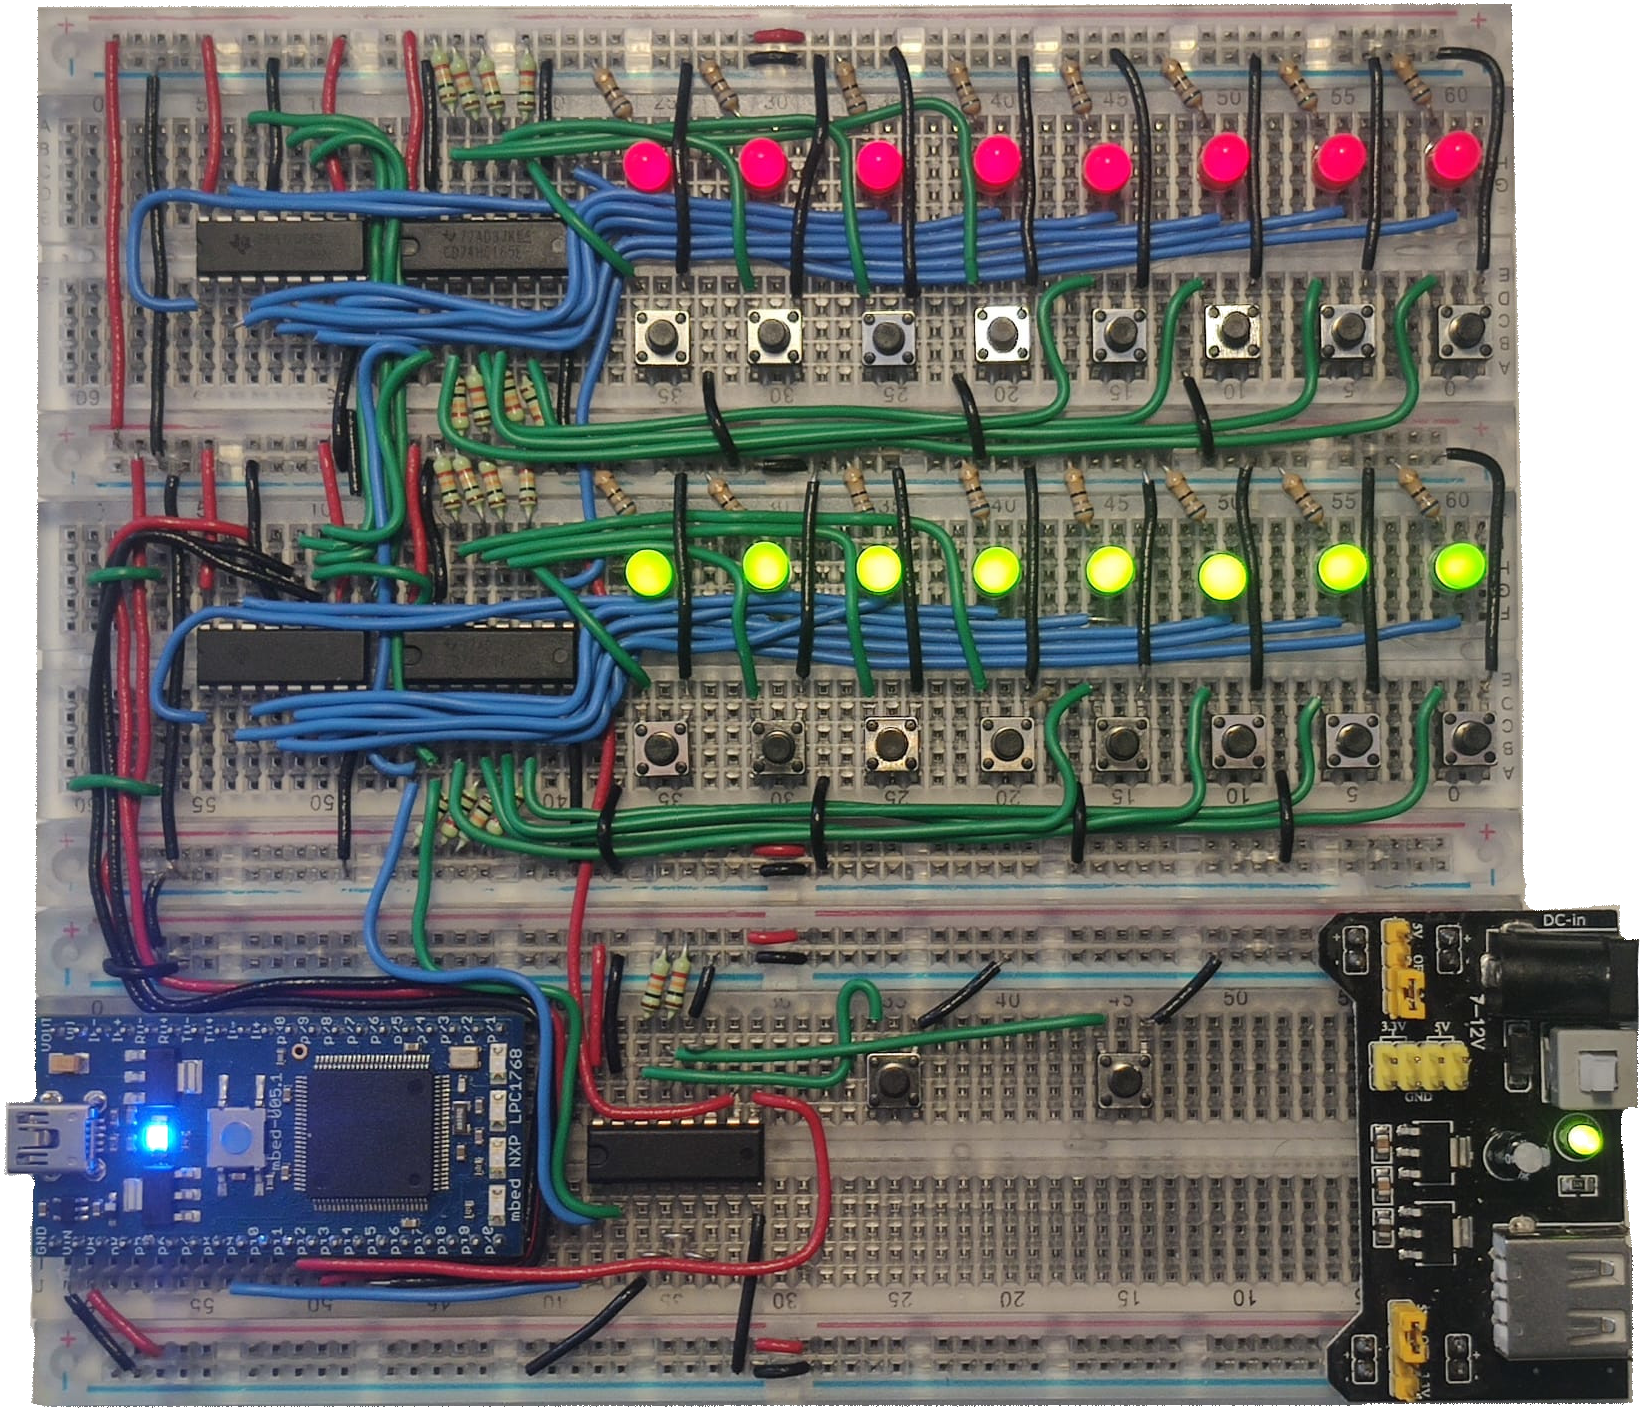
\includegraphics[width=.8\textwidth]{Cenital}}

    \caption{Prototype of a physical control panel}
    \label{fig:control_panel_proto}
\end{figure}

\section{Design}
\Gls{io} requirements for a control panel may easily overwhelm the pin count of any micro-controller. Therefore, several \gls{sipo} and \gls{piso} registers have been used to reduce the pin count to 4 outputs and 1 input. Moreover, using a discrete not logic gate, one of those outputs could be reused elsewhere. In total, 2 74HC595 8 bit \gls{sipo} registers are used to handle 16 \glspl{led}, whilst 3 74HC165 8 bit \gls{piso} registers are used for the 18 push-buttons. The implemented circuit diagram is shown in the figure \ref{fig:control_panel_proto_circuit}.\newline

\begin{sidewaysfigure}[hbtp]
    \centering
    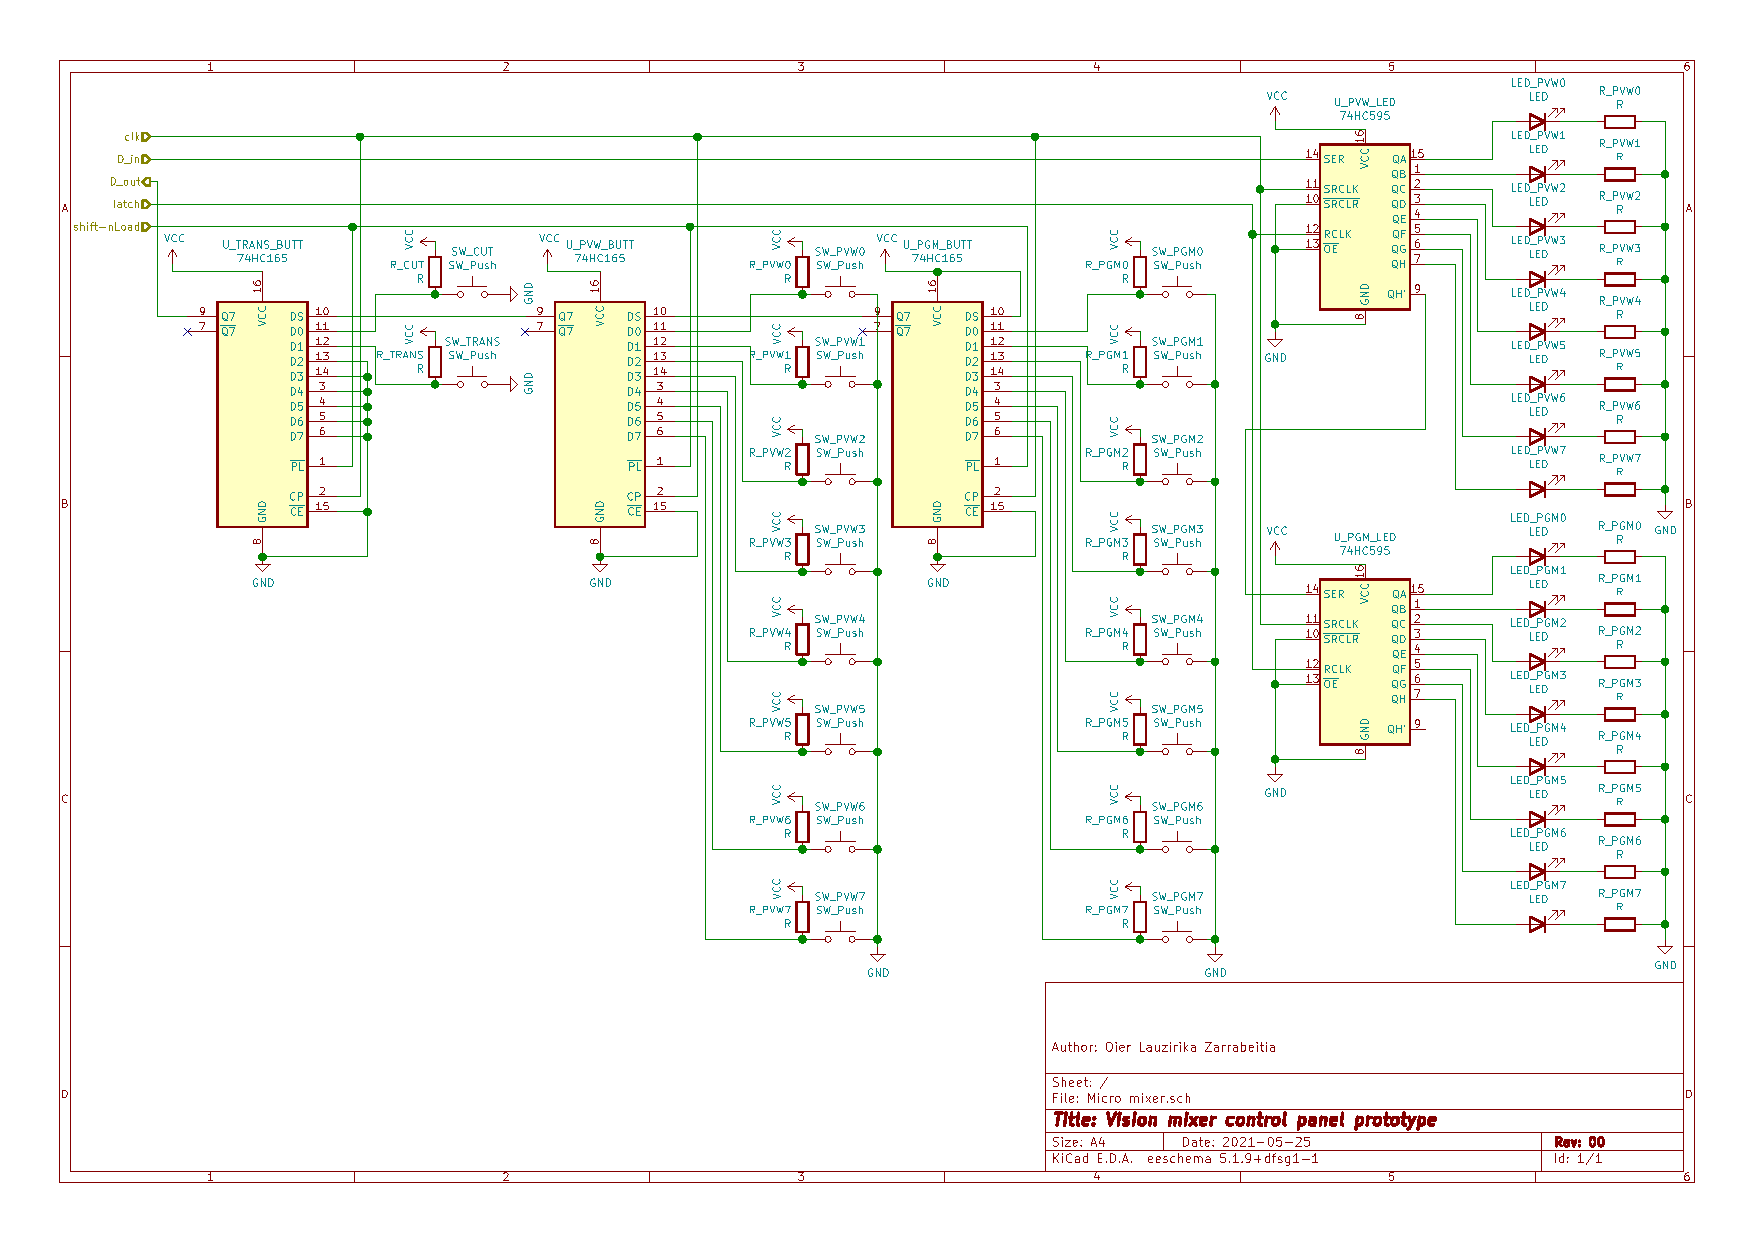
\includegraphics[width=\textwidth]{Circuit}

    \caption{Digital circuit blueprints for the control panel prototype}
    \label{fig:control_panel_proto_circuit}
\end{sidewaysfigure}


This control panel has been designed according to the competition's requirement of using a NXP LPC1768 microcontroller. However, in another context, this microcontroller should not be considered, as it is costly for the computational requirements of this control panel. The microcontroller only acts as a translation layer between the shift registers and the mixer. To communicate with the mixer, it uses the standard \gls{cli} protocol described in its corresponding appendix. However, these commands are transmitted using \gls{usart} over \gls{usb}. As the mixer does not support serial communications, a proxy must be set up, which forwards serial messages to a \gls{tcp} socket and vice versa.

\end{document}
